\documentclass[11pt]{article}
\usepackage[utf8]{inputenc}
\usepackage[T1]{fontenc}
\usepackage{url}
\usepackage{booktabs}
\usepackage{amsfonts}
\usepackage{nicefrac}
\usepackage{microtype}
\usepackage{fullpage}


\usepackage[numbers]{natbib}
%\usepackage[textsize=tiny]{todonotes}
\setlength{\marginparwidth}{11ex}

\newcommand{\E}{\mathbb E}
\usepackage{wrapfig}
\usepackage{caption}

\newcommand{\theHalgorithm}{\arabic{algorithm}}

\usepackage{url}

\usepackage[utf8]{inputenc}
\usepackage{amsmath}
\usepackage{graphicx}
\usepackage{upgreek}
\usepackage{amsfonts}
\usepackage{amssymb}
\usepackage{amsthm}
\usepackage[mathscr]{euscript}
\usepackage{mathtools}
\newtheorem{thm}{Theorem}
\newtheorem{defn}{Definition}
\newtheorem{cor}{Corollary}
\newtheorem{assumption}{Assumption}
\newtheorem{lem}{Lemma}
\usepackage{xcolor}
\usepackage{nicefrac}
\usepackage{xr}
%\usepackage{chngcntr}
\usepackage{apptools}
\usepackage[page, header]{appendix}
\AtAppendix{\counterwithin{lem}{section}}
\usepackage{titletoc}
\usepackage{enumitem}
\setlist[itemize]{leftmargin=1cm}
\setlist[enumerate]{leftmargin=1cm}



\definecolor{DarkRed}{rgb}{0.75,0,0}
\definecolor{DarkGreen}{rgb}{0,0.5,0}
\definecolor{DarkPurple}{rgb}{0.5,0,0.5}
\definecolor{Dark}{rgb}{0.5,0.5,0}
\definecolor{DarkBlue}{rgb}{0,0,0.7}
\usepackage[bookmarks, colorlinks=true, plainpages = false, citecolor = DarkBlue, urlcolor = blue, filecolor = black, linkcolor =DarkGreen]{hyperref}
\usepackage{breakurl}
\usepackage[ruled, vlined, linesnumbered]{algorithm2e}
\newcommand\mycommfont[1]{\footnotesize\ttfamily\textcolor{blue}{#1}}
\SetCommentSty{mycommfont}

\DeclareMathOperator*{\argmin}{arg\,min}
\DeclareMathOperator*{\argmax}{arg\,max}

\allowdisplaybreaks[2]
\newcommand{\prob}{\mathbb P}
\newcommand{\Var}{\mathbb V}
\newcommand{\Ex}{\mathbb E}
\newcommand{\varV}{\mathscr V}
\newcommand{\indicator}[1]{\mathbb I\{ #1 \} }
\newcommand{\statespace}{\mathcal S}
\newcommand{\actionspace}{\mathcal A}
\newcommand{\saspace}{\statespace \times \actionspace}
\newcommand{\satspace}{\mathcal Z}
\newcommand{\numsa}{\left|\saspace\right|}
\newcommand{\numsat}{\left|\satspace\right|}
\newcommand{\numS}{S}
\newcommand{\numA}{A}
\newcommand{\wmin}{w_{\min}}
\newcommand{\wminc}{w'_{\min}}
\newcommand{\range}{\operatorname{rng}}
\newcommand{\polylog}{\operatorname{polylog}}
\newcommand{\dspace}{\mathcal D}
\newcommand{\numD}{|\dspace|}
\newcommand{\numSucc}[1]{|\statespace(#1)|}
\newcommand{\succS}[1]{\statespace(#1)}

\newcommand{\reals}{\mathbb R}
\newcommand{\const}{\textrm{const.}}
\newcommand{\set}[1]{\left\{#1\right\}}
\newcommand{\llnp}{\operatorname{llnp}}
\newcommand{\defeq}{:=}
\usepackage{xspace}
\newcommand{\algname}{UBEV\xspace}

\mathtoolsset{showonlyrefs=true}

\let\temp\epsilon
\let\epsilon\varepsilon
\newcommand{\cK}{\mathcal K}
\newcommand{\cI}{\mathcal I}
\newcommand{\Pro}{\mathbb P}

\title{CS 234 Winter 2020 \\ Assignment 1 \\ Due: January 22 at 11:59 pm}
\date{}

\author{
  ksang\\
  \texttt{kaitoy@qq.com}
}

\begin{document}
	\maketitle
\noindent For submission instructions please refer to \href{http://web.stanford.edu/class/cs234/assignments.html}{website}.
For all problems, if you use an existing result from either the literature or a textbook to solve the exercise, you need to cite the source.




\section{Gridworld [15 pts]}

Consider the following grid environment. Starting from any unshaded square, you can move up, down, left, or right. Actions are deterministic and always succeed (e.g. going left from state 16 goes to state 15) unless they will cause the agent to run into a wall. The thicker edges indicate walls, and attempting to move in the direction of a wall results in staying in the same square (e.g. going in any direction other than left from state 16 stays in 16). Taking any action from the green target square (no. 12) earns a reward of $r_g$ (so $r(12, a)$ = $r_g$ $\forall a$) and ends the episode . Taking any action from the red square of death (no. 5) earns a reward of $r_r$ (so $r(5, a)$ = $r_r$ $\forall a$) and ends the episode. Otherwise, from every other square, taking any action is associated with a reward $r_s \in \{-1, 0, +1\}$ (even if the action results in the agent staying in the same square). Assume the discount factor $\gamma = 1$, $r_g = +5$, and $r_r = -5$ unless otherwise specified.

\begin{figure}[h]
  \centering
    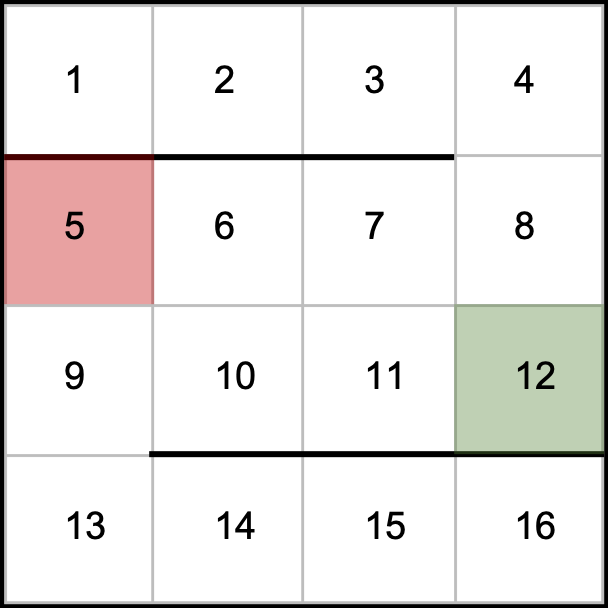
\includegraphics[width=0.3\textwidth]{tex/grid.png}
  	\label{fig:grid}
\end{figure}

\begin{enumerate}[label=(\alph*)]
\item (3pts) Define the value of $r_s$ that would cause the optimal policy to return the shortest path to the green target square (no. 12). Using this $r_s$, find the optimal value for each square.

\textbf{Answer:}

\begin{equation}
r_s = -1
\end{equation}

\begin{equation}
\begin{bmatrix}
0 & 1 & 2 & 3 \\
-5& 2 & 3 & 4 \\
2 & 3 & 4 & 5 \\
1 & 0& -1& -2
\end{bmatrix}
\end{equation}

\item (3pts) Lets refer to the value function derived in (a) as $V^{\pi_g}_{old}$ and the policy as $\pi_g$. Suppose we are now in a new gridworld where all the rewards ($r_s$, $r_g$, and $r_r$) have $+2$ added to them. Consider still following $\pi_g$ of the original gridworld, what will the new values $V^{\pi_g}_{new}$ be in this second gridworld?

\textbf{Answer:}

\begin{equation}
\begin{bmatrix}
12 & 11 & 10 & 9 \\
-3 & 10 & 9  & 8 \\
10 & 9  & 8  & 7 \\
11 & 12 & 13 & 14
\end{bmatrix}
\end{equation}

\item (3pts) Consider a general MDP with rewards, and transitions. Consider a discount factor of $\gamma$. For this case assume that the horizon is infinite (so there is no termination). A policy $\pi$ in this MDP induces a value function $V^\pi$ (lets refer to this as $V^\pi_{old}$). Now suppose we have a new MDP where the only difference is that all rewards have a constant $c$ added to them. Can you come up with an expression for the new value function $V^\pi_{new}$ induced by $\pi$ in this second MDP in terms of $V^\pi_{old}$, $c$, and $\gamma$?

\textbf{Answer:}

\begin{equation}
\begin{split}
V^\pi_{old}(s) & = \Ex_{\pi}[\sum_{t=0}^{\infty} \gamma^{t}r_t|s_0=s] \\
V^\pi_{new}(s) & = \Ex_{\pi}[\sum_{t=0}^{\infty}\gamma^{t}(r_t + c)|s_0=s] \\
               & = \Ex_{\pi}[\sum_{t=0}^{\infty}\gamma^{t}r_t|s_0=s] + c\sum_{t=0}^{\infty}\gamma^{t} \\
               & = V^\pi_{old}(s) + \frac{c}{1-\gamma}
\end{split}
\end{equation}



\item (2pts) Lets go back to our gridworld from (a) with the default values for $r_g$, $r_r$, $\gamma$ and with the value you specified for $r_s$. Suppose we now derived a second gridworld by adding a constant $c$ to all rewards ($r_s$, $r_g$, and $r_r$) such that $r_s = +2$. How does the optimal policy change (Just give a one or two sentence description)? What do the values of the unshaded squares become?

\textbf{Answer:}

It will become looping at states other than the terminate states, because each step will gain positive reward value.

Unshaded squares will become value $+\infty$.

\item (2pts) Now take the second gridworld from part (d) and change $\gamma$ such that $0 < \gamma < 1$. Can the optimal policy change and does it depend on your choice of gamma? (A brief description is sufficient, no formal proof or mathematical analysis required).

\textbf{Answer:}

If $\gamma$ is close to $1$, the result is same, all unshaded squares will have value $+\infty$ and optimal policy is keep looping.

if $\gamma$ is equal to some value closing to $0$, at some point optimal policy will be able to find a shortest path to green square.

\item (2pts) Lets go back to our gridworld from (a) with the default values for $r_g$, $r_r$, $\gamma$ and with the value you specified for $r_s$. In this gridworld, our optimal policy from any unshaded square never terminates in the red square. Now suppose $r_s$ can take on any real, non-infinite value and is not restricted to $\{+1, 0, -1\}$ anymore. Give a value of $r_s$ such that there are unshaded squares starting from which following the optimal policy results in termination in the red square.

\textbf{Answer:}

\begin{equation}
r_s \leq -5
\end{equation}


\end{enumerate}

\newpage
\section{Value of Different Policies [35 pts]}
In many situations such as healthcare or education, we cannot run any arbitrary policy and collect data from running those policies for evaluation. In these cases, we may need to take data collected from following one policy and use it to evaluate the value of a different policy. The equality proved in the following exercise can be an important tool for achieving this.
The purpose of this exercise is to get familiar on how to compare the value of different policies, $\pi_1$ and $\pi_2$, on a fixed horizon MDP. A fixed horizon MDP is an MDP where the agent's state is reset after $H$ timesteps; $H$ is called the \emph{horizon} of the MDP. There is no discount (i.e., $\gamma=1$) and policies are allowed to be non-stationary, i.e., the action identified by a policy depends on the timestep in addition to the state.
Let $x_t\sim \pi$ denote the distribution over states at timestep $t$ (for $1\leq t \leq H$) upon following policy $\pi$ and $V^{\pi}_t(x_t)$ denote the value function of policy $\pi$ in state 
$x_t$ and timestep $t$, and $Q_t^{\pi}(x_t,a)$ denote the corresponding 
$Q$ value associated to action $a$. As a clarifying example, we denote $\E_{x_t \sim \pi_1} V(x_t)$ to represent the average value of the value function $V(\cdot)$ over the states at timestep $t$ encountered upon following policy $\pi_1$. Please show the following:
\begin{equation}
\label{eq:1}
V_1^{\pi_1}(x_1) - V_1^{\pi_2}(x_1) =  \sum_{t=1}^H \E_{x_t \sim \pi_2} \Big( Q_t^{\pi_1}(x_t,\pi_1(x_t,t)) - Q_t^{\pi_1}(x_t,\pi_2(x_t,t)) \Big)
\end{equation}

\textbf{Intuition:} The above expression can be interpreted in the following way. For concreteness, assume that $\pi_1$ is the better policy, i.e., achieving $V_1^{\pi_1}(x_1) \geq V_1^{\pi_2}(x_1)$. Suppose you're following policy $\pi_2$ and you are at timestep $t$ in state $x_t$. 
You have the option to follow $\pi_1$ (the better policy) until the end of the episode, totalling $Q_t^{\pi_1}(x_t,\pi_1(x_t,t))$ return from the current state-timestep; or you have the option to follow $\pi_2$ for one timestep and then follow $\pi_1$ instead until the end of the episode (you can follow many other policies of course). This would you give you a ``loss'' of $Q_t^{\pi_1}(x_t,\pi_1(x_t,t)) - Q_t^{\pi_1}(x_t,\pi_2(x_t,t))$ that originates from following the worse policy $\pi_2$ instead of $\pi_1$ in that timestep. 
% Then equation \ref{eq:1} 
Then the equation above
means that the value difference of the two policies is the sum of all the losses induced by following the suboptimal policy for every timestep, weighted by the expected trajectory of the policy you're following.
\newpage
\section{Fixed Point [25 pts]}

In this exercise we will use  \href{https://en.wikipedia.org/wiki/Cauchy_sequence}{Cauchy sequences}  to prove that value iteration will converge to a unique fixed point (in this case, a value function $V$) regardless of the starting point. An element $V$ is a fixed point for an operator $B$ (in this case the Bellman operator) if performance of $B$ on $V$ returns $V$, i.e., $BV = V$. Recall that the Bellman backup operator $B$ is defined as (in lecture 2):
\begin{equation}
    V_{k+1} \overset{def}{=} BV_{k} = \max_a[ R(s, a) + \gamma\sum_{s' \in S}p(s'|s,a)V^\pi_{k}(s')].
\end{equation}

Additionally, in lecture 2, we proved that this Bellman backup is a contraction for $\gamma < 1$ on the infinity norm
\begin{equation}
    \|BV' - BV''\|_\infty\leq \gamma \|V' - V''\|_\infty
\end{equation}
for any two value functions $V'$ and $V''$, meaning if we apply it to two different value functions, the distance between value functions (in the $\infty$ norm) shrinks after application of the operator to each element.

\begin{enumerate}[label=(\alph*)]
\item (5pts) Prove by induction that $\|V_{n+1} - V_{n}\|_\infty \leq \gamma^n \|V_1 - V_0\|_\infty$

\textbf{Answer:}
\begin{equation}
\begin{aligned}
& n = 1: \\
& \|V_2 - V_1\|_\infty = \|BV_1 - BV_0\|_\infty\leq \gamma^1
\|V_1 - V_0\|_\infty \\
& n = 2: \\
& \|V_3 - V_2\|_\infty = \|BV_2 - BV_1\|_\infty\leq \gamma^1 \|V_2 - V_1\|_\infty \leq \gamma^1 \|V_1 - V_0\|_\infty \\
& n = k, \text{assume:} \\
& \|V_{k+1} - V_k\|_\infty \leq \gamma^1 \|V_1 - V_0\|_\infty \\
& \|V_{k+2} - V_{k+1}\|_\infty = \|BV_{k+1} - BV_k\|_\infty \\
& \leq \gamma^1\|V_{k+1} - V_k\|_\infty \leq \gamma^1 \gamma^k \|V_1 - V_0\|_\infty = \gamma^{k+1} \|V_1 - V_0\|_\infty \\
& 0 < \gamma < 1, \text{by induction: } \|V_{n+1} - V_{n}\|_\infty \leq \gamma \|V' - V''\|_\infty
\end{aligned}
\end{equation}


\item (10pts) Prove that for any $c>0$, $\|V_{n+c} - V_n\|_\infty \leq \frac{\gamma^n}{1-\gamma}\|V_1 - V_0\|_\infty$
\end{enumerate}

\textbf{Answer:}
\begin{equation}
\begin{aligned}
\text{consider } c > 1: &\\
\|V_{n+c} - V_n\|_\infty & = \|V_{n+c} - V_{n+1} + V_{n+1} - V_n\|_\infty \leq  \|V_{n+c} - V_{n+1}\|_\infty + \|V_{n+1} - V_n\|_\infty \\
\|V_{n+c} - V_n\|_\infty  & \leq \sum_{k=n}^{n+c}  \|V_{k+1} - V_k\|_\infty \\
                          & = \sum_{k=n}^{n+c} \gamma^k \|V_{1} - V_0\|_\infty \\
                          & = \frac{\gamma^n - \gamma^{n+c}}{1-\gamma}\|V_{1} - V_0\|_\infty \\
                          & \leq \frac{\gamma^n}{1-\gamma}\|V_{1} - V_0\|_\infty
\end{aligned}
\end{equation}

A \emph{Cauchy sequence} is a sequence whose elements become arbitrarily close to each other as the sequence progresses. Formally a sequence $\{a_n\}$ in metric space $X$ with distance metric $d$ is a Cauchy sequence if given an $\epsilon > 0$ there exists k such that if m, n > k then $d(a_m, a_n) < \epsilon$. Real Cauchy sequences are convergent.
\begin{enumerate}[label=(\alph*)]
\setcounter{enumi}{2}
\item (2pts) Using this information about Cauchy sequences, argue that the sequence $V_0, V_1, ...$ is a Cauchy sequence and is therefore convergent and must converge to some element $V$ and this V is a fixed point

\textbf{Answer:}
\begin{equation}
\text{let } k < n, m = n + c, \epsilon = \frac{\gamma^k}{1-\gamma}\|V_{1} - V_0\|_\infty:
\end{equation}
\begin{equation}
\begin{aligned}
\|V_{m} - V_n\|_\infty  & \leq \frac{\gamma^n}{1-\gamma}\|V_{1} - V_0\|_\infty \\
                          & < \frac{\gamma^k}{1-\gamma}\|V_{1} - V_0\|_\infty \\
                          & = \epsilon
\end{aligned}
\end{equation}

\item (8pts) Show that this fixed point is unique.

\end{enumerate}

Assume there are two fixed points $V$ and $V'$

At those points, because of convergence: $BV = V$

$\|V - V'\|_\infty = \|BV - BV'\|_\infty \leq \gamma \|V - V'\|_\infty$

Because $ 0 < \gamma < 1$, so $\|V - V'\| = 0$

Contraditon, there is only one fix point.

\newpage

\begin{section}{Frozen Lake MDP [25 pts]}
Now you will implement value iteration and policy iteration for the Frozen Lake environment
from \href{"https://gym.openai.com/envs/FrozenLake-v0"}{OpenAI Gym}. We have provided
custom versions of this environment in the starter code.
\begin{enumerate}[label=(\alph*)]

\item \textbf{(coding)} (10 pts) Read through \texttt{vi\_and\_pi.py} and implement \texttt{policy\_evaluation}, \texttt{policy\_improvement} and \texttt{policy\_iteration}. The stopping tolerance (defined as $\max_s |V_{old}(s) - V_{new}(s)|$) is tol = $10^{-3}$
. Use $\gamma = 0.9$. Return the optimal value function and the optimal policy.
\item \textbf{(coding)} (10 pts) Implement \texttt{value\_iteration} in \texttt{vi\_and\_pi.py}. The stopping tolerance is tol =
$10^{-3}$
. Use $\gamma = 0.9$. Return the optimal value function and the optimal policy.

\item \textbf{(written)} (5 pts) Run both methods on the Deterministic-4x4-FrozenLake-v0 and
Stochastic-4x4-FrozenLake-v0 environments. In the second environment, the dynamics of the world are stochastic. How does stochasticity affect the number of iterations required, and the resulting policy?

\textbf{Answer:}

Stocastic requires more iterations to converge, the resulting policy is same as dterministic one.

\end{enumerate}
\end{section}

\end{document}
